\documentclass[main.tex]{subfiles}
\begin{document}
	
	In this section, we present the initial results of our implementation of the GRIN framework. The measurements presented here can only be considered preliminary, given the compiler needs further work to be comparable to systems like the Glasgow Haskell Compiler or the Idris compiler~\cite{idris}. Nevertheless, these statistics are still relevant, since they provide valuable information about the effectiveness of the optimizer.
	
	\subsection{Measured programs}
	
	%TODO: include code of Length
	The measurements were taken using the Idris front end and LLVM back end of the compiler. Each test program --- besides ``Length" --- was adopted from the book \textit{Type-driven development with Idris}~\cite{tdd-idris} by Edwin Brady. These are small Idris programs demonstrating a certain aspect of the language.
	
	``Length" is an Idris program, calculating the length of a list containing the natural numbers from 1 to 100. This example was mainly constructed to test how the dead data elimination pass can transform the inner structure of a list into a simple natural number (see Section~\ref{sec:dde}).
	
	\subsection{Measured metrics}
	
	Each test program went trough the compilation pipeline described in Section~\ref{sec:idris-front-end}, and measurements were taken at certain points during the compilation. The programs were subject to three different types of measurements.
	
	\vspace{0.25cm}
	\begin{itemize}
		\item Static, compile time measurements of the GRIN code.
		\item Dynamic, runtime measurements of the interpreted GRIN code.
		\item Dynamic, runtime measurements of the executed binaries.
	\end{itemize}
	\vspace{0.25cm}

	The compile time measurements were taken during the GRIN optimization passes, after each transformation. The measured metrics were the number of \pilcode{store}s, \pilcode{fetch}es and function definitions. These measurements ought to illustrate how the GRIN code becomes more and more efficient during the optimization process. The corresponding diagrams for the static measurements are Diagrams~\ref{diagram:length-stats-ct}~to~\ref{diagram:reverse-stats-ct}. On the horizontal axis, we can see the indices of the transformations in the pipeline, and on the vertical axis, we can see the number of the corresponding syntax tree nodes. Reading these diagram from left to right, we can observe the continuous evolution of the GRIN program throughout the optimization process.
	
	The runtime measurements of the interpreted GRIN programs were taken at three points during the compilation process. First, right after the GRIN code is generated from the Idris byte code; second, after the regular optimization passes; and finally, at the end of the entire optimization pipeline. As can be seen on Figure~\ref{fig:idris-compilation-pipeline}, the regular optimizations are run a second time right after the dead data elimination pass. This is because the DDE pass can enable further optimizations. To clarify, the third runtime measurement of the interpreted GRIN program was taken after the second set of regular optimizations. The measured metrics were the number of executed function calls, case pattern matches, \pilcode{store}s and \pilcode{fetch}es. The goal of these measurements is to compare the GRIN programs at the beginning and at the end of the optimization pipeline, as well as to evaluate the efficiency of the dead data elimination pass. The corresponding diagrams for these measurement are Diagrams~\ref{diagram:length-stats-rt}~to~\ref{diagram:reverse-stats-rt}.

	The runtime measurements of the binaries were taken at the exact same points as the runtime measurements of the interpreted GRIN code. Their goal is similar as well, however they ought to compare the generated binaries instead of the GRIN programs. The measured metrics were the size of the binary, the number of executed user-space instructions, stores and loads. The binaries were generated by the LLVM back end described in Section~\ref{subsec:llvm-back-end} with varying opitmization levels for the LLVM Optimizer. The optimization levels are indicated in the corresponding tables: Tables~\ref{table:length-binary-results}~to~\ref{table:reverse-binary-results}. Where the optimization level is not specified, the default, \pilcode{O0} level was used. As for the LLVM Static Compiler and Clang, the most aggressive, \pilcode{O3} level was set for all the measurements.
	
	\subsection{Measurement setup}
	
	All the measurements were performed on a machine with \pilcode{Intel(R) Core(TM) i7-4710HQ CPU @ 2.50GHz} processor and \pilcode{Ubuntu 18.04 bionic} operating system with \pilcode{4.15.0-46-generic} kernel. The Idris compiler used by the front-end is of version 1.3.1, and the LLVM used by the back end is of version 7.
	
	The actual commands for the binary generation are detailed in Program~code~\ref{code:binary-gen}. That script has two parameters: \pilcode{N} and \pilcode{llvm-in}. \pilcode{N} is the optimization level for the LLVM Optimizer, and \pilcode{llvm-in} is the LLVM program generated from the optimized GRIN code.
	
	\vspace{-0.5cm}
	\begin{codeFloat}[h]
		\begin{bash}
			opt-7 -ON <llvm-in> -o <llvm-out> 
			llc-7 -O3 -relocation-model=pic -filetype=obj -o <object-file>
			clang-7 -O3 prim_ops.c runtime.c <object-file> -s -o <executable>
		\end{bash}
		\caption{Commands for binary generation}
		\label{code:binary-gen}
	\end{codeFloat}
	\vspace{-0.5cm}
	
	As for the runtime measurements of the binary, we used the \pilcode{perf} tool. The used command can be seen in Program~code~\ref{code:binary-measurements}.

	\vspace{-0.5cm}
	\begin{codeFloat}[h]
		\begin{bash}
			perf stat -e cpu/mem-stores/u -e "r81d0:u" -e instructions:u <executable>
		\end{bash}
		\caption{Command for runtime measurements of the binary}
		\label{code:binary-measurements}
	\end{codeFloat}
	\vspace{-0.5cm}
	
	
	\subsection{Length}
	
	The first thing we can notice on the runtime statistics of the GRIN code, is that the GRIN optimizer significantly reduced the number of heap operations, as well as the number of function calls and case pattern matches. Moreover, the DDE pass could further improve the program's performance by removing additional heap operations.
	
	The compile time statistics demonstrate an interesting phenomena. The number of \pilcode{store}s and function definitions continuously keep decreasing, but at a certain point, the number of \pilcode{fetch}es suddenly increase by a relatively huge margin. This is due to the fact that the optimizer usually performs some preliminary transformations on the GRIN program \emph{before} inlining function definitions. This explains the sudden rise in the number of \pilcode{fetch}es during the early stages of the optimization process. Following that spike, the number of heap operations and function definitions gradually decrease until the program cannot be optimized any further.
	
	\begin{figure}[h]
		\hspace{-0.5cm}
		\renewcommand{\figurename}{Diagram}
		\caption{Length - GRIN statistics}
		\label{diagram:length-stats}
		\addtocounter{figure}{-1}
		\begin{minipage}{0.5\textwidth}
			\subcaption{Runtime}
			\label{diagram:length-stats-rt}
			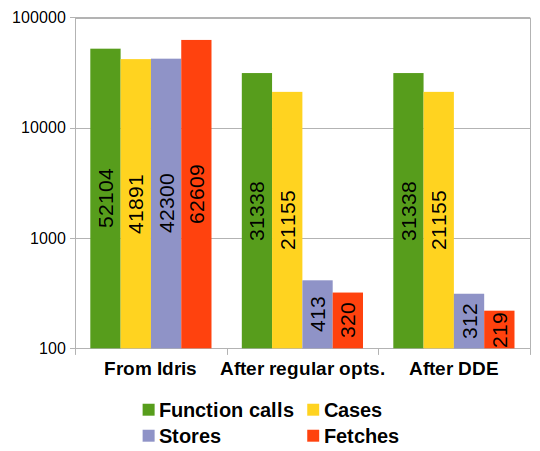
\includegraphics[scale=0.43]{length-runtime.png}
		\end{minipage}
		\begin{minipage}{0.5\textwidth}
			\subcaption{Compile time}
			\label{diagram:length-stats-ct}
			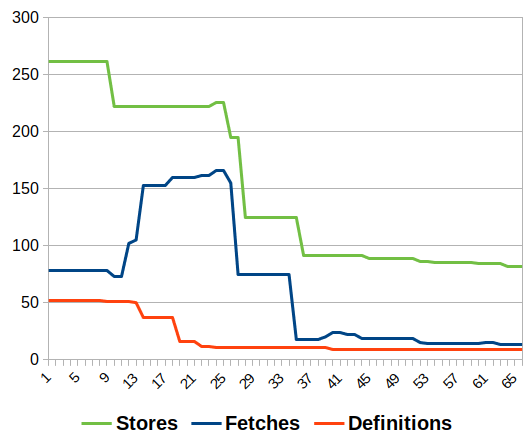
\includegraphics[scale=0.43]{length-compile-time.png}
		\end{minipage}
	\end{figure}

	The runtime statistics for the executed binary are particularly interesting. First, observing the \pilcode{O0} statistics, we can see that the regular optimizations substantially reduced the number of executed instructions and memory operations, just as we saw with the interpreted GRIN code. However, on the one hand the DDE optimized binary did not perform any better than the regularly optimized one, but on the other hand its size decreased by more than 20\%. 
	
	\begin{center}
		\begin{minipage}{0.74\linewidth}
			\captionof{table}{Length - CPU binary statistics}
			\label{table:length-binary-results}
			\begin{tcolorbox}[tab2,tabularx={l||r|r|r|r}]
				Stage                 & Size  & Instructions & Stores & Loads      \\
				\hline\hline
				\pilcode{normal-O0}   & 23928 & 769588 & 212567 & 233305 \\\hline
				\pilcode{normal-O3}   & 23928 & 550065 & 160252 & 170202 \\\hline
				\pilcode{regular-opt} & 19832 & 257397 & 14848  & 45499  \\\hline
				\pilcode{dde-O0}      & 15736 & 256062 & 14243  & 45083  \\\hline
				\pilcode{dde-O3}      & 15736 & 284970 & 33929  & 54555  \\
			\end{tcolorbox}	
		\end{minipage}
	\end{center}
	
	Also, it is interesting to see that the aggressively optimized DDE binary performed much worse than the \pilcode{O0} version. This is because the default optimization pipeline of LLVM is designed for the C and C++ languages. As a consequence, in certain scenarios it may perform poorly for other languages. In the future, we plan to construct a better LLVM optimization pipeline for GRIN.

	\subsection{Exact length}
	
	For the GRIN statistics of ``Exact length", we can draw very similar conclusions as for ``Length``. However, closely observing the statistics, we can see, that the DDE pass completely eliminated \emph{all} heap operations from the program. In principle, this means, that all the variables can be put into registers during the execution of the program. In practice, some variables will be spilled onto stack, but the heap will never be used.

	\begin{figure}[h]
		\hspace{-0.5cm}
		\renewcommand{\figurename}{Diagram}
		\caption{Exact length - GRIN statistics}
		\label{diagram:exact-length-stats}
		\addtocounter{figure}{-1}
		\begin{minipage}{0.5\textwidth}
			\subcaption{Runtime}
			\label{diagram:exact-length-stats-rt}
			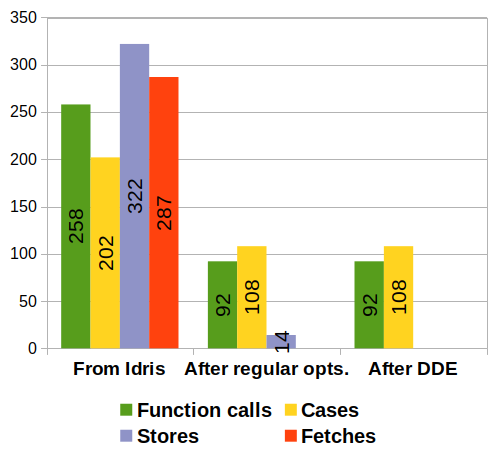
\includegraphics[scale=0.43]{exact-length-runtime.png}
		\end{minipage}
		\begin{minipage}{0.5\textwidth}
			\subcaption{Compile time}
			\label{diagram:exact-length-stats-ct}
			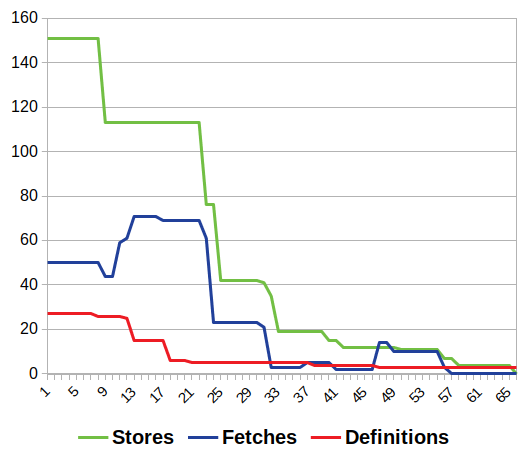
\includegraphics[scale=0.43]{exact-length-compile-time.png}
		\end{minipage}
	\end{figure}

	As for the binary statistics, we do not see any major improvements besides the significant reduction in the size of the binary. Although, it is worth pointing out, that the cost of memory operations can be considerably higher when accessing heap memory, and that the statistics presented here do not account for that.

	\begin{center}
		\begin{minipage}{0.72\linewidth}
			\captionof{table}{Exact length - CPU binary statistics}
			\label{table:exact-length-binary-results}
			\begin{tcolorbox}[tab2,tabularx={l||r|r|r|r}]
				Stage                 & Size  & Instructions & Stores & Loads      \\
				\hline\hline
				\pilcode{normal-O0}   & 18800 & 188469 & 14852 & 46566 \\\hline
				\pilcode{normal-O3}   & 14704 & 187380 & 14621 & 46233 \\\hline
				\pilcode{regular-opt} & 10608 & 183560 & 13462 & 45214 \\\hline
				\pilcode{dde-O0}      & 10608 & 183413 & 13431 & 45189 \\\hline
				\pilcode{dde-O3}      & 10608 & 183322 & 13430 & 44226 \\
			\end{tcolorbox}	
		\end{minipage}
	\end{center}

	\newpage
	\subsection{Type level functions}
	
	The GRIN statistics for this program may not be particularly interesting, but they demonstrate that the GRIN optimizations work for programs with many type level computations as well.
	
	\begin{figure}[h]
		\hspace{-0.5cm}
		\renewcommand{\figurename}{Diagram}
		\caption{Type level functions - GRIN statistics}
		\label{diagram:tyfuns-stats}
		\addtocounter{figure}{-1}
		\begin{minipage}{0.5\textwidth}
			\subcaption{Runtime}
			\label{diagram:tyfuns-stats-rt}
			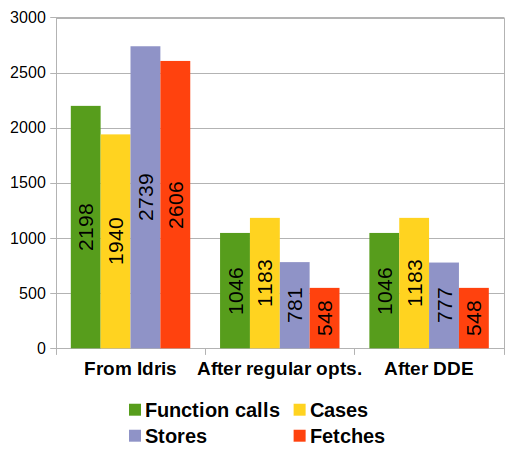
\includegraphics[scale=0.43]{tyfuns-runtime.png}
		\end{minipage}
		\begin{minipage}{0.5\textwidth}
			\subcaption{Compile time}
			\label{diagram:tyfuns-stats-ct}
			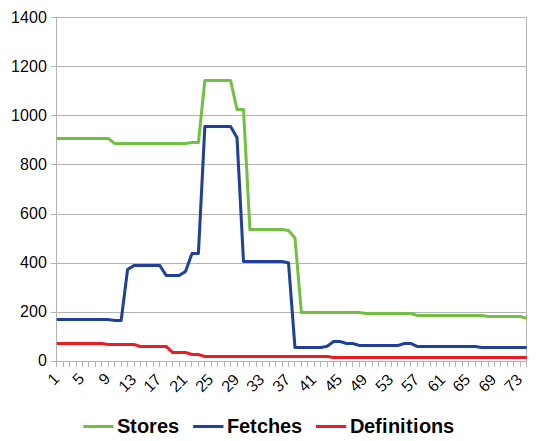
\includegraphics[scale=0.43]{tyfuns-compile-time.png}
		\end{minipage}
	\end{figure}

	The binary statistics look promising for ``Type level functions". Each measured performance metric is strictly decreasing, which suggests that even the default LLVM optimization pipeline can work for GRIN.

	\begin{center}
		\begin{minipage}{0.72\linewidth}
			\captionof{table}{Type level functions - CPU binary statistics}
			\label{table:tyfuns-binary-results}
			\begin{tcolorbox}[tab2,tabularx={l||r|r|r|r}]
				Stage                 & Size  & Instructions & Stores & Loads      \\
				\hline\hline
				\pilcode{normal-O0}   & 65128 & 383012 & 49191 & 86754 \\\hline
				\pilcode{normal-O3}   & 69224 & 377165 & 47556 & 84156 \\\hline
				\pilcode{regular-opt} & 36456 & 312122 & 34340 & 71162 \\\hline
				\pilcode{dde-O0}      & 32360 & 312075 & 34331 & 70530 \\\hline
				\pilcode{dde-O3}      & 28264 & 309822 & 33943 & 70386 \\
			\end{tcolorbox}	
		\end{minipage}
	\end{center}

	\subsection{Reverse}
	
	Unlike, the previous programs, ``Reverse" could not have been optimized by the dead data elimination pass. The pass had no effect on it. Fortunately, the regular optimizations alone could considerably improve both the runtime and compile time metrics of the GRIN code.
	
	The binary statistics are rather promising. The binary size decreased by a substantial margin and the number of executed memory operations has also been reduced by quite a lot.
	
	\begin{figure}[h]
		\hspace{-0.5cm}
		\renewcommand{\figurename}{Diagram}
		\caption{Reverse - GRIN statistics}
		\label{diagram:reverse-stats}
		\addtocounter{figure}{-1}
		\begin{minipage}{0.5\textwidth}
			\subcaption{Runtime}
			\label{diagram:reverse-stats-rt}
			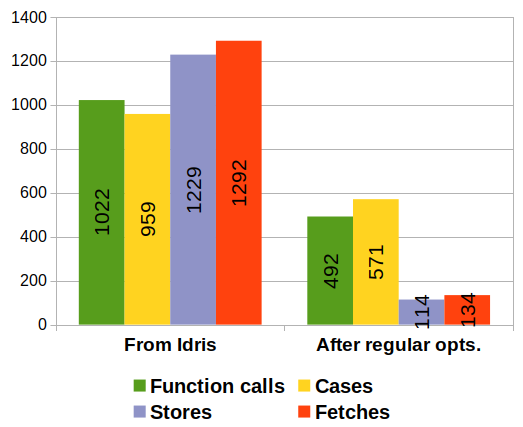
\includegraphics[scale=0.43]{reverse-runtime.png}
		\end{minipage}
		\begin{minipage}{0.5\textwidth}
			\subcaption{Compile time}
			\label{diagram:reverse-stats-ct}
			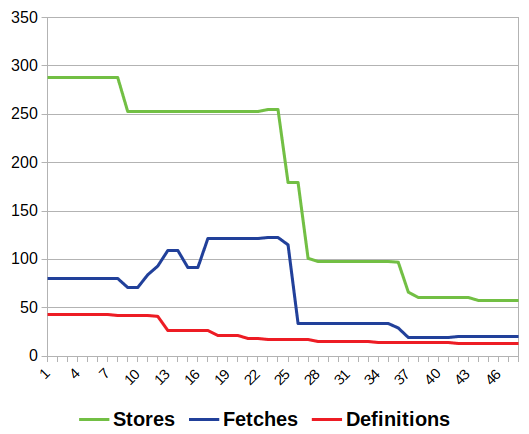
\includegraphics[scale=0.43]{reverse-compile-time.png}
		\end{minipage}
	\end{figure}
	
	\begin{center}
		\begin{minipage}{0.76\linewidth}
			\captionof{table}{Reverse - CPU binary statistics}
			\label{table:reverse-binary-results}
			\begin{tcolorbox}[tab2,tabularx={l||r|r|r|r}]
				Stage                 & Size  & Instructions & Stores & Loads      \\
				\hline\hline
				\pilcode{normal-O0}      & 27112 & 240983 & 25018 & 58253 \\\hline
				\pilcode{normal-O3}      & 31208 & 236570 & 23808 & 56617 \\\hline
				\pilcode{regular-opt-O0} & 14824 & 222085 & 19757 & 53125 \\\hline
				\pilcode{regular-opt-O3} & 14824 & 220837 & 19599 & 52827 \\
			\end{tcolorbox}	
		\end{minipage}
	\end{center}

	\subsection{General conclusions}
	
	In general, the measurements demonstrate that the GRIN optimizer can considerably improve the performance metrics of a given GRIN program. The regular optimizations themselves can usually produce highly efficient programs, however, in certain cases the dead data elimination pass can facilitate additional optimizations, and can further improve the performance.
	
	The results of the binary measurements indicate that the GRIN optimizer performs optimizations orthogonal to the LLVM optimizations. This supports the motivation behind the framework, which is to transform functional programs into a more manageable format for LLVM by eliminating the functional artifacts. This is backed up by the fact, that none of the fully optimized \pilcode{normal} programs could perform as well as the regularly or DDE optimized ones. Also, it is interesting to see, that there is not much difference between the \pilcode{O0} and \pilcode{O3} default LLVM optimization pipelines for GRIN. This motivates further research to find an optimal pipeline for GRIN. 
	
	Finally, it is rather surprising to see, that the dead data elimination pass did not really impact the performance metrics of the executed binaries, but it significantly reduced their size. The former can be explained by the fact, that most of these programs are quite simple, and do not contain any compound data structures. Dead data elimination can shine when a data structure is used in a specific way, so that it can be locally restructured for each use site. However, when applying it to simple programs, we can obtain sub par results.

\end{document}